\begin{comment}\documentclass[14pt]{article}
\usepackage{fullpage}
\usepackage{tabularx}
\usepackage{array}
\usepackage{tikz}
\usetikzlibrary{positioning,arrows.meta,bending,automata}
\usepackage{amsfonts}
\usepackage{setspace}
\usepackage{geometry}
\usepackage{verbatim}
\geometry{paperwidth=2000mm, paperheight=800pt, left=40pt, top=40pt, textwidth=2000mm, marginparsep=20pt, marginparwidth=100pt, textheight=16263pt, footskip=40pt}
\begin{document}
\end{comment}
\def\arraystretch{1.5}
\tikzstyle{every picture}+=[remember picture]
\begin{tabular}{l|l|c|c}
& \verb~(gotoifnot ? 1)~ &
&
\\
& \verb~2:~ & 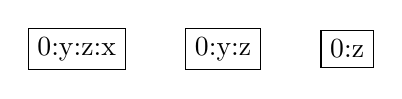
\begin{tikzpicture}[baseline=-2pt]
\node[draw] (phi16_ref1) { 0:y:z:x };
\node[draw,right=5ex of phi16_ref1] (phi16_ref3) { 0:y:z };
\node[draw,right=5ex of phi16_ref3] (phi16_ref5) { 0:z };
\end{tikzpicture}
&
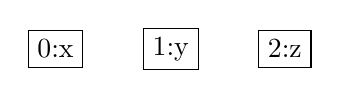
\begin{tikzpicture}[baseline=-2pt]
\node[draw] (phi16_ref2) { 0:x };
\node[draw,right=5ex of phi16_ref2] (phi16_ref4) { 1:y };
\node[draw,right=5ex of phi16_ref4] (phi16_ref6) { 2:z };
\end{tikzpicture}

\\
& \verb~z~ & 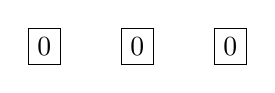
\begin{tikzpicture}[baseline=-2pt]
\node[draw] (pc17ref1) { 0 };
\node[draw,right=5ex of pc17ref1] (pc17ref2) { 0 };
\node[draw,right=5ex of pc17ref2] (pc17ref3) { 0 };
\end{tikzpicture}
&
\begin{tikzpicture}[baseline=-2pt]
\node (d0) {};
\node[draw,right=6em of d0] (pc17ref4) { 2 };
\end{tikzpicture}
\begin{tikzpicture}[overlay]
\draw[->,thick,black] (pc17ref1) edge (phi16_ref1);
\draw[->,thick,black] (pc17ref2) edge (phi16_ref3);
\draw[->,thick,black] (pc17ref3) edge (phi16_ref5);
\draw[->,thick,black] (pc17ref4) edge (phi16_ref6);
\end{tikzpicture}
\\
& \verb~y~ & 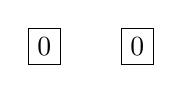
\begin{tikzpicture}[baseline=-2pt]
\node[draw] (pc18ref1) { 0 };
\node[draw,right=5ex of pc18ref1] (pc18ref2) { 0 };
\end{tikzpicture}
&

\begin{tikzpicture}[baseline=-2pt]
\node[draw] (pc18ref3) { 1 };
\end{tikzpicture}
\begin{tikzpicture}[overlay]
\draw[->,thick,black] (pc18ref1) edge (pc17ref1);
\draw[->,thick,black] (pc18ref2) edge (pc17ref2);
\draw[->,thick,black] (pc18ref3) edge (phi16_ref4);
\end{tikzpicture}
\\
& \verb~x~ & 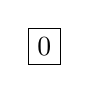
\begin{tikzpicture}[baseline=-2pt]
\node[draw] (pc19ref1) { 0 };
\end{tikzpicture}
&
\begin{tikzpicture}[baseline=-2pt]
\node (d0) {};
\node[draw,left=6em of d0] (pc19ref2) { 0 };
\end{tikzpicture}
\begin{tikzpicture}[overlay]
\draw[->,thick,black] (pc19ref1) edge (pc18ref1);
\draw[->,thick,black] (pc19ref2) edge (phi16_ref2);
\end{tikzpicture}
\\ 
& \verb~y~ & 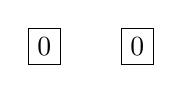
\begin{tikzpicture}[baseline=-2pt]
\node[draw] (pc21ref1) { 0 };
\node[draw,right=5ex of pc21ref1] (pc21ref2) { 0 };
\end{tikzpicture}
&
\begin{tikzpicture}[baseline=-2pt]
\node (d) {};
\node[draw,right=6em of d] (pc21ref3) { 1 };
\end{tikzpicture}
\begin{tikzpicture}[overlay]
\draw[->,thick,black] (pc21ref1) edge (pc19ref1);
\draw[->,thick,black] (pc21ref2) edge (pc18ref2);
\draw[->,thick,black] (pc21ref3) edge (pc18ref3);
\end{tikzpicture}
\\
& \verb~(= z y)~ & 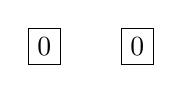
\begin{tikzpicture}[baseline=-2pt]
\node[draw] (pc22ref1) { 0 };
\node[draw,right=5ex of pc22ref1] (pc22ref2) { 0 };
\end{tikzpicture}
&
\begin{tikzpicture}[baseline=-2pt]
\node (d) {};
\node[draw,right=6em] (pc22ref3) { 1 };
\end{tikzpicture}
\begin{tikzpicture}[overlay]
\draw[->,thick,black] (pc22ref1) edge (pc21ref1);
\draw[->,thick,black] (pc22ref2) edge (pc21ref2);
\draw[->,thick,black] (pc22ref3) edge (pc21ref3);
\end{tikzpicture}
\\
& \verb~x~ & 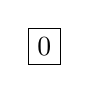
\begin{tikzpicture}[baseline=-2pt]
\node[draw] (pc24ref1) { 0 };
\end{tikzpicture}
&
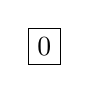
\begin{tikzpicture}[baseline=-2pt]
\node[draw] (pc24ref2) { 0 };
\end{tikzpicture}
\begin{tikzpicture}[overlay]
\draw[->,thick,black] (pc24ref1) edge (pc22ref1);
\draw[->,thick,black] (pc24ref2) edge (pc19ref2);
\end{tikzpicture}
\\
& \verb~(= y x)~ & 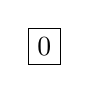
\begin{tikzpicture}[baseline=-2pt]
\node[draw] (pc25ref1) { 0 };
\end{tikzpicture}
&
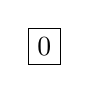
\begin{tikzpicture}[baseline=-2pt]
\node[draw] (pc25ref2) { 0 };
\end{tikzpicture}
\begin{tikzpicture}[overlay]
\draw[->,thick,black] (pc25ref1) edge (pc24ref1);
\draw[->,thick,black] (pc25ref2) edge (pc24ref2);
\end{tikzpicture}
\\
& \verb~(new)~ & \begin{tikzpicture}[baseline=-2pt]
\end{tikzpicture}
&
\begin{tikzpicture}[baseline=-2pt]
\node (d) {};
\node[draw,left=6em of d] (pc30ref1) { 0 };
\end{tikzpicture}
\begin{tikzpicture}[overlay]
\end{tikzpicture}
\\
& \verb~(= x (new))~ & \begin{tikzpicture}[baseline=-2pt]
\end{tikzpicture}
&
\begin{tikzpicture}[baseline=-2pt]
\node (d) {};
\node[draw,left=6em of d] (pc31ref1) { 0 };
\end{tikzpicture}
\begin{tikzpicture}[overlay]
\draw[->,thick,black] (pc31ref1) edge (pc30ref1);
\end{tikzpicture}
\\
& \verb~z~ & 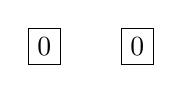
\begin{tikzpicture}[baseline=-2pt]
\node[draw] (pc172ref1) { 0 };
\node[draw,right=5ex of pc172ref1] (pc172ref2) { 0 };
\end{tikzpicture}
&
\begin{tikzpicture}[baseline=-2pt]
\node (d0) {};
\node[draw,right=6em of d0] (pc172ref4) { 2 };
\end{tikzpicture}
\begin{tikzpicture}[overlay]
\draw[->,thick,black] (pc172ref1) edge (pc25ref1);
\draw[->,thick,black] (pc172ref2) edge (pc22ref2);
\draw[->,thick,black] (pc172ref4) edge (pc22ref3);
\end{tikzpicture}
\\
& \verb~y~ & 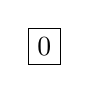
\begin{tikzpicture}[baseline=-2pt]
\node[draw] (pc182ref1) { 0 };
\end{tikzpicture}
&

\begin{tikzpicture}[baseline=-2pt]
\node[draw] (pc182ref3) { 1 };
\end{tikzpicture}
\begin{tikzpicture}[overlay]
\draw[->,thick,black] (pc182ref1) edge (pc172ref1);
\draw[->,thick,black] (pc182ref3) edge (pc25ref2);
\end{tikzpicture}
\\
& \verb~x~ & \begin{tikzpicture}[baseline=-2pt]
\end{tikzpicture}
&
\begin{tikzpicture}[baseline=-2pt]
\node (d0) {};
\node[draw,left=6em of d0] (pc192ref2) { 0 };
\end{tikzpicture}
\begin{tikzpicture}[overlay]
\draw[->,thick,black] (pc192ref2) edge (pc31ref1);
\end{tikzpicture}
\\ 
 & \verb~(gotoifnot (! ?) 2)~ & \begin{tikzpicture}[baseline=-2pt]
\end{tikzpicture}
&
\\
& \verb~1:~ & 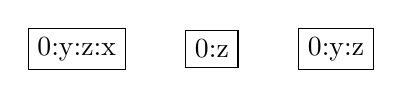
\begin{tikzpicture}[baseline=-2pt]
\node[draw] (phi36_ref1) { 0:y:z:x };
\node[draw,right=5ex of phi36_ref1] (phi36_ref5) { 0:z };
\node[draw,right=5ex of phi36_ref5] (phi36_ref6) { 0:y:z };
\end{tikzpicture}
&
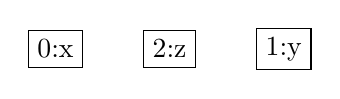
\begin{tikzpicture}[baseline=-2pt]
\node[draw] (phi36_ref2) { 0:x };
\node[draw,right=5ex of phi36_ref2] (phi36_ref3) { 2:z };
\node[draw,right=5ex of phi36_ref3] (phi36_ref4) { 1:y };
\end{tikzpicture}
\\
\end{tabular}
%\end{document}
